\chapter{Experimental setup}
\label{Experiment}
The \gls{LHC} successfully began circulating its first protons within its 27 km long underground tunnel on the 10th of September 2008.  
Unfortunately an incident on the 19th of that same month where a magnet quench caused 6 tonnes of liquid helium to vent and subsequently expand with violent force damaged over 50 superconducting magnets which needed to be repaired.   
On the 23rd of November the following year the first collisions were recorded~\cite{FirstCollisions}, signalling the beginning of the LHC era at the forefront of the high energy frontier.  
In the years since the LHC has been consistently pushing to more frequent collisions at higher energies, allowing the experiments along its ring to explore and extend our knowledge of physics at the subatomic level.  

This chapter describes the technology that allows these studies to be performed.  
First a description of the LHC acceleration complex is provided.  
This is followed by a subdetector by subdetector description of the ATLAS detector, including details on the physics behind the technology used in these detectors.  

\section{The Large Hadron Collider}
\label{Sec:LHC}

The components of a particle accelerator can be grouped into two functional categories: rf cavities which use electric fields to accelerate particles, and magnets which are used to control the accelerated particles.  
Circular accelerators come in two distinct types: cyclotrons which contain the beam using a fixed-strength magnetic field but allow for the radius of the charged particles' orbit to increase, and synchrotrons which maintain a fixed radius by increasing the magnetic field strength to compensate for the increasing energy of the accelerating particles.  
The LHC fits into the second of these categories.  

Designing a single synchrotron accelerator to accelerate bunches of protons to the energies attained at the LHC would be a difficult and expensive task.
One requirement would be the ability to finely control the field in the superconducting electromagnets used to contain the particle beam in the ring over several orders of magnitude of energy.  
A much more cost effective approach involves using existing machines to accomplish at least part of this task, and that's exactly the approach used at the LHC.  

The LHC acceleration complex begins with a linear accelerator, called linac2, a machine that accelerates protons originating from and ion source to 50 MeV in bunches.  
These bunches are delivered to the PS booster, a machine that consists of four superimposed synchrotron rings which accelerate protons to 1.4 GeV before they are injected into the next machine, the Proton Synchrotron.  
The Proton Synchrotron, or PS, is the oldest component of the LHC acceleration facility.  
It was built in the 1950's and was designed to accelerate up to 10$^{10}$ protons per pulse to 26 GeV.

After the PS, the protons are injected into the Super Proton Synchrotron (SPS), a machine that in 1976 when it was turned on had the ability to accelerate protons to 400 GeV, the second highest energy attainable by an accelerator at that time.  
The SPS, while in proton/anti-proton collision mode (the so-called Sp$\bar{\mathrm p}$S mode) allowed the discovery of both the W and Z bosons by the UA1 and UA2 collaborations.  
It may be worth noting that it takes several fills of the PS to fill the SPS, and it subsequently takes several fills of the SPS to fully fill the LHC.  
The SPS is now the final pre-injector into the LHC, accelerating the protons up to 450 GeV before they enter the LHC itself.  

The LHC is a machine that was designed to use 16 RF cavities to accelerate 2808 bunches, each with 1.15x$10^{11}$ protons, to 7 TeV per proton.  
These bunches travel the 27~km around the ring of the LHC being held in orbit by 1232 superconducting dipole magnets (8.33 Tesla) which bend the beam, along with a number of additional magnets, mostly quadruples, which help focus the beam~\cite{LHCTDR}.  
The LHC then crosses these counter rotating beams at four points along the beam line (the four experiments listed in~\ref{Sec:Experi}) every 25 ns, with an average of 25 interactions occurring per crossing (up to $\sim$ 52) in 2016. 

One measure of the collider's performance is its luminosity, a description of the number of particles per unit area per unit time, which directly relates to the number of collisions per unit time and therefore the probability of obtaining a given final state.  
The LHC's design luminosity is approximately 20 times the maximum luminosity of its predecessor, the Tevatron ($10^{34}$ cm$^{-2}$s$^{-1}$ vs. 4 x $10^{32}$ cm$^{-2}$s$^{-1}$), with this design luminosity being surpassed by the end of the 2016 data taking period (1.38 x $10^{34}$ cm$^{-2}$s$^{-1})$. 

\section{The ATLAS Experiment}
\label{Sec:ATLAS}

\subsection{The ATLAS Coordinate System}

The origin of the coordinate system that is used in ATLAS is at the geometric centre of the ATLAS detector.  
The z-axis is parallel to the beam pipe running counterclockwise along the LHC ring when viewed from above, with the x-axis pointing toward the middle of the ring and the y-axis pointing up.  
A more common way to describe the coordinates in the x-y plane is to use the azimuthal angle $\phi$, where $\phi$=0 is defined to be along the positive x-axis and to increase in the direction of the positive y-axis, along with the radial coordinate $r$ which is the distance of the point from the origin.  
As the remnants of the collisions will be ejected in all directions a spherical coordinate system is adopted by adding a second angle $\theta$, with the most natural orientation being to define $\theta$=0 being in the x-y plane with $\theta$ increasing in the direction of the positive z-axis.  
When it comes to high energy physics however it is often more convenient to speak in terms of rapidity($y$) and pseudorapidity($\eta$).  
This is especially true for a hadron collider like the LHC, which at high energy effectively collides partons.  
Within the protons each parton carries an unknown fraction of the total momentum of the proton.  
This means that the center of mass frame for each collision is Lorentz boosted along the $z$ axis.  
This makes the use of $\theta$ problematic due to how it transforms as one transitions from the detector reference frame to the centre of mass reference frame.  
Rapidity, given by $y=\frac{1}{2}\mathrm{ln}\left[\frac{E+p_{z}}{E-p_z}\right]$, is much more helpful in this regard as differences in rapidity remain constant under Lorentz boosts.  
Pseudorapidity, defined as $\eta=-\mathrm{ln}\left[\mathrm{tan}\left(\frac{\theta}{2}\right)\right]$, is a good approximation for rapidity, especially at high energy, and does not require knowledge of the energy and momentum of the particle in question.  
Pseudorapidity is equal to the rapidity in the case of a massless particle.  

\begin{figure}[!ht]
  \begin{center}
    \scalebox{0.153}{
      \includegraphics[angle =90]{plots/Chap2/ATLAS_detector_alles_mittel_EN.ps}
    }
  \end{center}
  \caption[Layout of the ATLAS detector]
  {\small Layout of the ATLAS detector showing the location of the various subdetectors.  ATLAS Experiment Image: Copyright CERN,~\cite{Pequenao:1095924}.}
\end{figure}

\subsection{ATLAS Detector: Overview}

ATLAS is a multipurpose detector, meaning it must be able to simultaneously measure the large number and variety of particles produced in each collision provided by the LHC at a high enough rate to take advantage of the large luminosity required for the physics studies at the LHC. 
The ATLAS detector is composed of many individual layers, with each layer being designed to measure different properties of the particles.  
Going from the interaction point outwards these layers are known as the inner detector, the electromagnetic (EM) calorimeter, the hadronic calorimeter, and the muon spectrometer.   

\begin{figure}[!ht]
  \begin{center}
    \scalebox{0.08}{
      \includegraphics{plots/Chap2/ID.ps}
    }
  \end{center}
  \caption[Layout of the ATLAS Inner Detector]
  {\small Drawing of the various subsystems of the inner detector.  ATLAS Experiment Image: Copyright CERN,~\cite{Pequenao:1095926}.}
\end{figure}

\subsection{ATLAS Hardware: Inner Detector}
\label{Sec.ID}
The inner detector is made up of three subdetectors: the pixel detector, the \gls{SCT}, and the \gls{TRT}.  
These three subdetectors are all immersed in a 2 Tesla magnetic field that is supplied by a solenoidal magnet.  
This magnetic field bends the trajectories of charged particles by an amount that is proportional to their momentum.  
The main purpose of the inner detector is to make non destructive measurements of this bending, allowing the momentum of charged particles to be measured.  
It is also possible to track the trajectories of multiple particles back to a single origin, called a vertex.  
Vertices along the beam axis may indicate an individual proton-proton collision event, while vertices off of the beam axis may indicate the location where some heavy particle produced in the original collision further decays into lighter secondaries.  
The \gls{TRT} also contributed to particle identification by measuring transition radiation (discussed later in this section).  
 
These trajectories are measured by a large number of concentric cylindrical detectors (and circular endcap detectors)  with well known positions surrounding the interaction point.  
When a particle passes through these detectors a space-point is measured (a hit).  
A pattern recognition, or reconstruction, algorithm is then run over all of these hits to recreate the paths the particles have travelled (known as tracks).  
It is this track reconstruction that leads the inner detector to more colloquially be known as the tracker.  

The first two subdetectors of the tracker are both semiconductor detectors, a type of detector that measures the electron-hole pairs that are produced as a charged particle passes through silicon sensors that are segmented into either squares (pixels) or strips.  
Both are made up of 4 concentric cylinders in the central region, and circular endcap disks further extending the $\eta$ coverage of the detectors.  
For the 2011 and 2012 data taking periods the pixel detector consisted of three layers situated a radial distance of 50.5, 88.5 and 122.5 mm from the centre of the beam pipe.  
The layers are made up of 22, 38 and 52 staves, with each stave containing 6 x $10^5$ pixels.  
This detector is capped at both ends by three endcap disk layers, with each endcap having a further 4.4 x $10^6$ pixels.  
The resolution of a tracking detector is parameterized by A $\oplus$ B/p$_{\mathrm{T}}$, where A is the intrinsic resolution of the detector and B describes the effect of multiple scatterings on the resolution.  
This setup allowed for an intrinsic resolution of 10 $\mu$m in the transverse impact parameter d$_{0}$ and 115 $\mu$m in the longitudinal impact parameter (z$_{0}$ sin$\theta$)~\cite{ID3}, which are measures of the distance from the particle track to the reconstructed vertex. 

\begin{figure}[!ht]
 \begin{center}
 \scalebox{0.3}{
  \includegraphics{plots/Chap2/FigID26-mod-011107.ps}
 }
 \end{center}
 \caption[Layout and coverage of the ID]
 {\small Layout and coverage of the ID.  Figure from ~\cite{Iwamoto:2013kla}}
 \label{IDCoverage}
\end{figure} 

During the first long shutdown of the LHC a fourth additional layer was added closer to the beam, known as the \gls{IBL}.  
This layer was designed to deal with the high occupancy expected as the luminosity delivered by the LHC increases into 2020 (2-3 x $10^{34}$ cm$^{-2}$s$^{-1}$)~\cite{IBL1}, and to provide an additional hit near the interaction point to ensure good tracking efficiency as the ID ages.  
This new layer has 14 staves which are arranged in an overlapping circular pattern 33~mm away from the centre of the beam pipe, adding a further 6x10$^6$ individual readout pixels to the pixel detector.
The IBL improves the intrinsic resolution of the pixel detector by a factor of 1.7~in longitudinal impact parameter and by 1.2~in transverse impact parameter.  
It also reduces the $p_{\mathrm T}$ dependence of the resolution by a factor of 1.8 in both directions~\cite{IBL2}.  
One measurement that can be improved by this increased track resolution is b-tagging, which involves using vertices which are displaced from the beam line to identify the remnants of very short lived particles decaying before they reach the tracking system (in this case b mesons).  
The light jet rejection rate of a b-tagger set to accept 60\% of b jets has been shown to increase by nearly a factor of 2 with this improvement in resolution (in the absence of pileup).

As mentioned above the SCT is also a semiconductor detector, consisting of 4088 mod- ules tiling 4 cylinders and two endcaps, with each endcap consisting of 9 layers~\cite{JOIATLAS}.  
In the barrel these modules consist of two inner and two outer sensors with a stereo angle of 40 mrad to provide a position measurement in a complemantary direction.  
The endcap modules use the same strategy, having two sensors glued back-to-back once again with a stereo angle of 40~mrad.  
The SCT has a nominal resolution of 17~$\mu$m in R-$\phi$ and 580~$\mu$m in z.  

The final subsystem in the tracker is the TRT which uses up to 73 layers of gas filled ``straws'' in the barrel and as many as 160 straw planes in the endcaps.  
Each straw is filled with a mixture of 70\% xenon gas (for x-ray absorption), 27\% CO2, and 3\% O2 (for increasing the electron drift velocity and photon quenching).  
Charged particles ionize the gas mixture as they pass through and the charge is collected by a central gold plated tungsten anode wire within each straw.  
Each of these 144~cm long straws provides only information in R-$\phi$, for which the intrinsic accuracy is 130~$\mu$m.  
In addition to providing position measurements the TRT is also able to detect the low energy transition radiation photons created as the charged particles travel between the gas, the layers within the straw walls, and the inter-straw medium (polypropylene foils or fibres).  
The amount of radiation emitted during each transition is a function of the Lorentz factor of the particle.  
By having two detection thresholds for each straw, a low ionization threshold and a high transition radiation threshold, and counting the number of high threshold hits belonging to a given reconstructed track, information about the type of particle creating the track can be obtained.  
Tracks with a large number of high threshold hits can be assumed to be highly boosted light particles, namely electrons.  

\subsection{ATLAS Hardware: Calorimeter}
Calorimeters, in contrast to tracking systems, absorb the energy of incoming particles through destructive processes and produce signals that are proportional to the initial incoming energy.  
In addition to pure energy measurements calorimeters which are segmented into $\eta$ x $\phi$ x $R$ cells can also provide information on how the energy from a given particle is deposited, which helps both particle identification and energy calibration.  
With a large coverage in both $\eta$ and $\phi$ one can also determine the location in $\phi$ where signals may be expected due to the conservation of momentum in the transverse plane but nothing is detected.  
These imbalances in measured momentum may interpreted as a miscalibration of the observed energy or as particles having passed through the detector without interacting such as a neutrino.

The ATLAS calorimeter is broken up into three $\eta$ sections: the central barrel region, the endcaps and the forward calorimeters (FCal).  
In all three regions the ATLAS calorimeter is split into two well defined primary longitudinal segments, the \gls{EM} calorimeter, and the hadronic calorimeter.   
This division is to take advantage of the relatively shallow showering depth of electromagnetic particles while ensuring that the much deeper hadronic showers are still fully measured.  
These differences will be further explained in the following sections.  

The remainder of this section is divided into four subsections.  
The first subsection describes particles which result in electromagnetic showers and how electromagnetic showers are propagated.  
This is followed by a description of the technology used in the EM calorimeters in ATLAS.  
The same two stage approach is also used to explain hadronic showers and how they are measured in ATLAS.  

\subsubsection{Electromagnetic Calorimeter}
\label{EMCalo} 

Electromagnetic calorimeters are focused on measuring the energy of photons and electrons, which interact with matter through a variety of processes which are all results of the electromagnetic interaction~\cite{grupen2008particle}~\cite{Wigmans2008}.  
The photon for example has four primary processes through which it interacts with matter: Rayleigh scattering, the photoelectric effect, Compton scattering, and pair production.  
The contribution of each of these processes to the overall energy loss of the photon depends on the energy of the photon.  

\begin{figure}[!ht]
    \begin{center}
      \scalebox{0.5}{
        \includegraphics{plots/Chap2/PhotonInteractionCrossSectionInLead.ps}
      }
    \end{center}
        \caption[Contributions to the photon interaction cross section]
        {\small Contributions to the photon interaction cross section as a function of the photon energy.  $\tau$ is the photoelectric effect, $\sigma_{\mathrm{COH}}$ is Rayleigh scattering, $\sigma_{\mathrm{INCOH}}$ is Compton scattering, $\kappa_{\mathrm n}$ and $\kappa_{\mathrm e}$ is pair production off of atomic nuclei and electrons respectively in lead~\cite{:/content/aip/journal/jpcrd/9/4/10.1063/1.555629}. 
}
            \label{Photon}
\end{figure}

For low energy photons (less than $\sim$ 100 KeV) the photoelectric effect, where a photon is absorbed by an atom and an electron is emitted, dominates.  
Due to the strong energy dependence of the cross section for this process (goes as E$^{-3}$) it is largely suppressed for higher energy photons.   
Rayleigh scattering, which is the coherent scattering of photons by atomic nuclei and is the second most important process at low energy, also dies out very quickly with increasing photon energies.  
In most materials for photons with energies between $\mathcal{O}\mathrm(10 \mathrm{KeV})$ to $\mathcal{O}\mathrm(10 \mathrm{MeV})$ the largest contribution to the photon interaction cross section is Compton scattering.  
In Compton scattering photons scatter from atomic electrons.  
%a portion of the photon's energy is used to excite an atomic electron into an unbound state.  
For even larger energies the dominant interaction mechanism is pair production where a photon, while interacting with the EM field of either an atomic nucleus or an electron, creates an electron/positron pair.  
Pair production is possible for photons with energies above twice the mass of an electron (2 x 511 KeV), with the cross section growing rapidly before leveling off at higher energies.  
Figure~\ref{Photon} shows the cross-section for these various interaction mechanisms for photons in lead.  
An important measure of the number of interactions a photon will experience while travelling through a material is the mean distance traveled between each interaction, or the mean free path ($\lambda\left(E\right)$).  
By measuring the amount of material present in a given detector in terms of $\lambda$ one can more readily compare two calorimeters made with different materials.  


The primary electromagnetic mechanism through which charged particles (electrons and positrons for example) lose their energy is also energy dependent.  
Lower energy particles primarily lose energy by ionizing the material they are travelling through (with processes like M{\o}ller scattering or Bhabha scattering also contributing).  
Particles with higher energy tend to lose energy by radiating photons (bremsstrahlung).  
The energy at which the average energy loss due to ionization is equal to the average energy loss due to bremsstrahlung is called the critical energy $\epsilon_{\mathrm{C}}$.  
The critical energy depends both on the atomic number Z of the material, and more strongly, on the mass of the particle in question.  
The critical energy is proportional to m$^2$, meaning that for energies typically reached in experiment the bremsstrahlung component to the energy loss can be insignificant for particles with masses even as low as 100 MeV (muons and pions for example).  
While photons are usually discussed in terms of mean free path, electron interactions with matter are characterized by the energy lost per unit distance which is also a function of energy($-\frac{dE}{dx}=\frac{E}{\chi_{0}}$).  
$\chi_{0}$, known as the radiation length, defines this energy loss rate and is the average distance an electron will travel before radiating a photon.  

\begin{figure}[!ht]
  \begin{center}
    \scalebox{0.5}{
      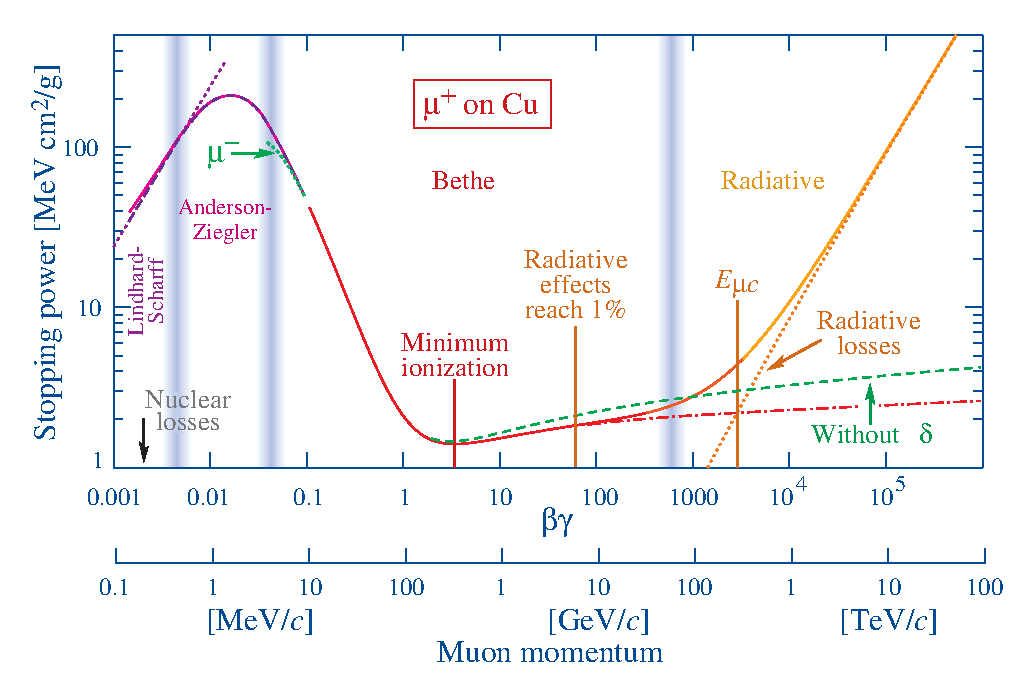
\includegraphics{plots/Chap2/rpp_icru49_cu_col.eps}
    }
  \end{center}
  \caption[Stopping power for positive muons in copper.]
  {\small Stopping power ($\frac{-dE}{dx}$) for positive muons in copper as a function of $\beta\gamma=\frac{p}{Mc}$, see ref.~\cite{PDG}.  Here $\delta$ is to account for the muon polarizing the material near itself which screens out charges further from the away from the muon (dependent on density).  } 
  \label{StoppingMuon}
\end{figure}

The dominant interaction mechanism for high energy photons is pair production, which results in a high energy electron/positron pair, and light high energy charged particles lose energy primarily by emitting photons.  
With this in mind it is easy to imagine that a single high energy EM particle will lead to a large cascade of lower energy EM particles while travelling through a material.  
These cascading events (known as electromagnetic showers) tend to remain in a narrow cone around the trajectory of the initiating particle, with the tightness of the cone being independent of the initial energy of the particle (see Moli{\`e}re radius in~\cite{grupen2008particle}).  
Another feature of electromagnetic showers is that, relatively speaking, they do not penetrate very deeply into the material.   
These are properties that will be useful in identifying EM showers.  
See Sec.~\ref{EMReco}. 

\begin{table}
  \centering
  \begin{tabular}{ |c|c|c|}
  \hline
  \multicolumn{3}{|c|}{\textbf{EM calorimeter}} \\
  \hline
  \hline
  \multicolumn{3}{|c|}{Longitudinal layers, $\eta$ coverage} \\
  \hline
  Presampler  & 1, $\mid\eta\mid<1.52$            & 1, $1.5<\mid\eta\mid<1.8$ \\
  \hline
  Calorimeter & 3, $\mid\eta\mid<1.35$            & 2, $.1375<\mid\eta\mid1.5$ \\
              & 2, $1.35<\mid\eta\mid<1.475$      & 3, $1.5<\mid\eta\mid<2.5$ \\
              &                                   & 2, $2.5<\mid\eta\mid<3.2$ \\
  \hline
  FCal        &                                   & 1, $3.1<\mid\eta\mid < 4.9$ \\
  \hline
  \multicolumn{3}{|c|}{Granularity $\Delta\eta x \Delta\phi$} \\
  \hline
  Presampler  & 0.025 x 0.1, $\mid\eta\mid<1.52$                & 0.025 x 0.1, $1.5<\mid\eta\mid<1.8$ \\
  \hline
  Calorimeter layer 1 & 0.003 x 0.1, $\mid\eta\mid<1.4$         & 0.05 x 0.1,  $1.375<\mid\eta\mid<1.425$ \\
                      & 0.025 x 0.025, $1.4<\mid\eta\mid<1.475$ & 0.025 x 0.1, $1.425<\mid\eta\mid<1.5$ \\
                      &                                         & 0.003 x 0.1, $1.5<\mid\eta\mid<1.8$ \\
                      &                                         & 0.004 x 0.1, $1.8<\mid\eta\mid<2.0$ \\
                      &                                         & 0.006 x 0.1, $2.0<\mid\eta\mid<2.4$ \\
                      &                                         & 0.025 x 0.1, $2.4<\mid\eta\mid<2.5$ \\
                      &                                         & 0.1 x 0.1,   $2.5<\mid\eta\mid<3.2$ \\
  \hline
  Calorimeter layer 2 & 0.025 x 0.025, $\mid\eta\mid<1.4$       & 0.05 x 0.025,$1.375<\mid\eta\mid<1.425$ \\
                      & 0.075 x 0.025, $1.4<\mid\eta\mid<1.475$ & 0.025 x 0.025, $1.425<\mid\eta\mid<2.5$ \\
                      &                                         & 0.1 x 0.1, $2.5<\mid\eta\mid<3.2$ \\
  \hline
  Calorimeter layer 3 & 0.05 x 0.025, $\mid\eta\mid<1.35$       & 0.05 x 0.025, $1.5<\mid\eta\mid<2.5$ \\
  \hline
  FCal                &                                         & 0.2 x 0.2, $3.1<\mid\eta\mid < 4.9$ \\
  \hline
  \end{tabular}
  \caption[Main parameters of the electromagnetic calorimeter system. ]
        {\small Main parameters of the electromagnetic calorimeter system in ATLAS~\cite{JOIATLAS} }
\label{table:EMCalo}
\end{table}

The ATLAS detector makes use of sampling calorimeters.  
In a sampling calorimeter a dense material used to create the particle shower (absorber) alternates with an active material that measures the energy deposited.  
While there is a disadvantage to this design with energy deposited in the absorber being invisible to the detector, having the full energy of the particle being deposited in a shorter length of material allows for a reduction in size of any additional detectors beyond the calorimeter.  
It is also typically cheaper.  
In both the barrel and endcaps the absorber for the EM calorimeter is lead and the active material is liquid argon (LAr), while in the forward region a copper/LAr combination is used.  
When charged particles, both primary and secondary, pass through the active medium the liquid argon is ionized and the charge is collected on kapton electrodes.  
A breakdown of how the number of sampling layers and the resolution of the EM calorimeter vary with $\eta$ in the central and endcap regions is shown in Table~\ref{table:EMCalo}.  

\begin{figure}[!ht]
  \begin{center}
    \scalebox{0.08}{
      \includegraphics{plots/Chap2/ATLAS_Calo.ps}
    }
  \end{center}
  \caption[Layout of the ATLAS Calorimeters]
  {\small Computer generated image showing how the various subsystems of the ATLAS calorimeter are arranged.  ATLAS Experiment Image: Copyright CERN,~\cite{Pequenao:1095927}.}
\end{figure}


\subsubsection{Hadronic Calorimeter}
\label{Had}
There are many similarities between EM calorimeters and hadronic calorimeters.  
Hadronic calorimeters rely on both electromagnetic and nuclear interactions between the particles to be measured and the detector.  
These interactions produce secondary particles, which go on to have subsequent interactions with the material in the calorimeter.  
This process, known as a hadronic shower, continues until the secondary particles reach a low enough energy that they are fully absorbed by the material and their energy is measured through ionization.  
The differences between hadronic and electromagnetic showers are the size of the shower, both in depth and width (with hadronic showers being larger in both dimensions) and the event by event variations of the showers (with hadronic showers being subject to much larger fluctuations because of the large number of available types and the character of nuclear interactions).  


As the lowest mass charged hadron is over 200 times more massive than the electron ($\pi^{\pm}$ at 140 MeV) it is safe to assume that at energies which will be achieved in the ATLAS detector bremsstrahlung will not be an important energy loss mechanism for hadrons.  
Ionization and excitation on the other hand are still relevant contributors to the overall energy loss of hadrons.  
The rate at which energy is lost via these mechanisms for particles which are heavier than an electron is described by the Bethe-Bloch formula,  
\begin{equation}
-\frac{\mathrm{d}E}{\mathrm{d}x}=\frac{2CZz^2}{A\beta^2}\left[\mathrm{ln}\left(a\gamma^2\beta^2\right)-\beta^2-\frac{\delta}{2}\right], 
\end{equation}
where $C$ is a constant, $z$ is the charge of the incident particle, $Z$ and $A$ are the atomic number and weight of the material being ionized, $\beta$ and $\gamma$ are the velocity and Lorentz factors of the incident particle, $\delta$ is a parameter describing density effects, and $a$ depends on the electron mass and the ionization energy of the absorber.  

While these particles do interact electromagnetically it is the interactions between the hadrons and the atomic nuclei via the nuclear force (resulting in secondary hadrons) that account for the majority of the energy loss.  
The average distance between these interactions is much larger than the radiation length which is the cause of the extra penetration depth of these showers compared to EM showers.  
To get an idea of the difference in length of hadronic and electromagnetic showers one needs only to pick a material, say copper, and compare the hadronic interaction length $\lambda_{\mathrm{int}}$ (15 cm in copper) to the radiation length $\chi_{0}$ in the same material (1.4 cm)~\cite{Wigmans2008}.  
The large width of hadronic showers is caused by large transverse momentum transfer in the nuclear interactions.  

\begin{table}
  \centering
  \begin{tabular}{ |c|c|c|}
  \hline
  \multicolumn{3}{|c|}{\textbf{Hadronic calorimeter}} \\
  \hline
  \hline
  \multicolumn{3}{|c|}{Tile calorimeter} \\
  \hline 
                     & Barrel                                   & Extended barrel \\
  Coverage           & $\mid\eta\mid<1.0$                       & $0.8<\mid\eta\mid<1.7$ \\
  \hline 
  Number of layers   & 3                                        & 3 \\
  \hline 
  Granularity        & 0.1 x 0.1				& 0.1 x 0.1 \\
  Last layer only    & 0.2 x 0.1				& 0.2 x 0.1 \\
  \hline 
  \hline
  \multicolumn{3}{|c|}{Hadronic endcaps} \\
  \hline 
  Coverage           & 	\multicolumn{2}{|c|}{$1.5<\mid\eta\mid<3.2$} \\
  \hline
  Number of layers   &  \multicolumn{2}{|c|}{ 4} \\
  \hline
  Granularity        & 	\multicolumn{2}{|c|}{0.1 x 0.1, $1.5<\mid\eta\mid<2.5$} \\
  		     &  \multicolumn{2}{|c|}{ 0.2 x 0.2, $2.5<\mid\eta\mid<3.2$} \\
  \hline
  \hline
  \multicolumn{3}{|c|}{Forward calorimeter} \\
  \hline
  Coverage	     & \multicolumn{2}{|c|}{$3.1<\mid\eta\mid<4.9$} \\
  \hline
  Number of layers   & \multicolumn{2}{|c|}{2} \\
  \hline
  Granularity        & \multicolumn{2}{|c|}{$\approx$ 0.2 x 0.2} \\
  \hline
  \end{tabular}
  \caption[Main parameters of the hadronic calorimeter system. ]
        {\small Main parameters of the hadronic calorimeter system in ATLAS~\cite{JOIATLAS}. }
%1748-0221-3-08-S08003} }
\label{table:HadCalo}
\end{table}

While a large fraction of the particles resulting from the nuclear interactions is pions ($\approx$ 90 \%), other particles like protons, neutrons, kaons, etc. are also produced.  
On average the three pion flavours ($\pi^0$, $\pi^{+}$, and $\pi^{-}$) are produced with equal frequency, with large variations being possible between any two given interactions.  
Charged pions interact with matter much differently than their neutral counterparts.  
Where charged pions have a mean lifetime $\tau$ of 2.6 x $10^{-8}$ s ($c\tau$ = 7.8 m) and tend to have further nuclear interactions before decaying, neutral pions have a much shorter lifetime ($c\tau$ = 25 nm) and quickly decay into a pair of photons which initiate EM showers within the hadronic shower~\cite{PDG}.  
As a result of this important difference the amount of detectable energy deposited in a calorimeter from a hadronic shower can have a strong dependence on the fraction of neutral pions from the first few interactions.  

The fraction of the total energy deposited in the calorimeter by these small EM sub-showers ($f_{em}$) varies as a function of the energy of the particle initiating the shower, increasing from $\approx$ 30\% for particles at 10 GeV to $\approx$ 50\% for particles at 100 GeV.  
The rest of the energy can be accounted for as follows: 34\% is used to overcome the nuclear binding potential to release protons and neutrons (so called invisible energy), 10\% is in low energy (typically 3 MeV) neutrons which have been released from nuclear spallation reactions, and 56\% is deposited via ionizing particles, where 2/3 of that is via protons~\cite{Wigmans2008}.  
Therefore, a large portion of the non-EM energy is deposited in the calorimeter via low energy free nucleons, not relativistic pions.  

The hadronic calorimeter is also a sampling calorimeter.  
The similarities with the EM calorimeter go even further in that in both the FCal and endcaps the active material for the hadronic calorimeter is LAr, with the absorber in the endcaps being copper and the absorber in the forward region being tungsten.  
In the barrel the hadronic calorimeter uses steel as the absorber material and plastic scintillator as the active material.  
The number of sampling layers and the granularity of each of the regions of the hadronic calorimeter are shown in Table.~\ref{table:HadCalo}. 


\begin{figure}[!ht]
  \begin{center}
    \scalebox{0.4}{
      \includegraphics{plots/Chap2/0803022_01.ps}
    }
  \end{center}
  \caption[Grafic showing different particle interactions]
      {\small Cross-section of the muon system in a plane containing the beam axis (bending plane). The muon track bends in the magnetic field of the ID and deposits small amounts of energy in every detector along it's path.  Note that muons are the only charged particles to reach the muon spectrometer~\cite{JOIATLAS}.}
  \label{MuonSpectroFig}
\end{figure}


\subsection{ATLAS Hardware: Muon Spectrometer}

Muons are 200 times heavier than electrons, are typically minimum ionizing at the LHC (see Fig.~\ref{StoppingMuon}) and therefore do not produce electromagnetic showers.  
Since muons also do not interact via the nuclear force, they do not produce hadronic showers either.  
Thankfully as they are charge carriers they do interact with the tracking systems in the inner detector, and with the help of a second tracking system beyond the hadronic calorimeter they are easy to identify as they are the only ionizing particles that regularly pass through the entire calorimeter.  
The magnetic field for the muon spectrometer is provided by large superconducting air-core toroids, with the field in the central region ($\mid\eta\mid$< 1.4) being provided by the barrel toroid and in the forward regions (1.6 <$\mid\eta\mid$< 2.7) by two relatively smaller endcap magnets.  
In the transition regions the magnetic fields are provided by a combination of these three magnets.  

In the central barrel region the muon hits are measured in three separate layers (stations) that are arranged in concentric cylinders with radii of about 5, 7.5, and 10~m~\cite{MuonTDR}.  
These distances are chosen to measure the muons' position as they enter, are at the midpoint, and again as they exit the magnetic field to best measure the deflection of the muons and hence their momentum.  
The two endcaps consist of four wheels at distances of 7.4, 10.8, 14, and 21.5~m from the interaction point. 
The additional wheel at 10.8~m is to allow for the full three measurements of the muon trajectory in the region that is uncovered by the outermost wheel (see Fig.~\ref{MuonSpectroFig}).


\begin{figure}[!ht]
  \begin{center}
    \scalebox{0.4}{
      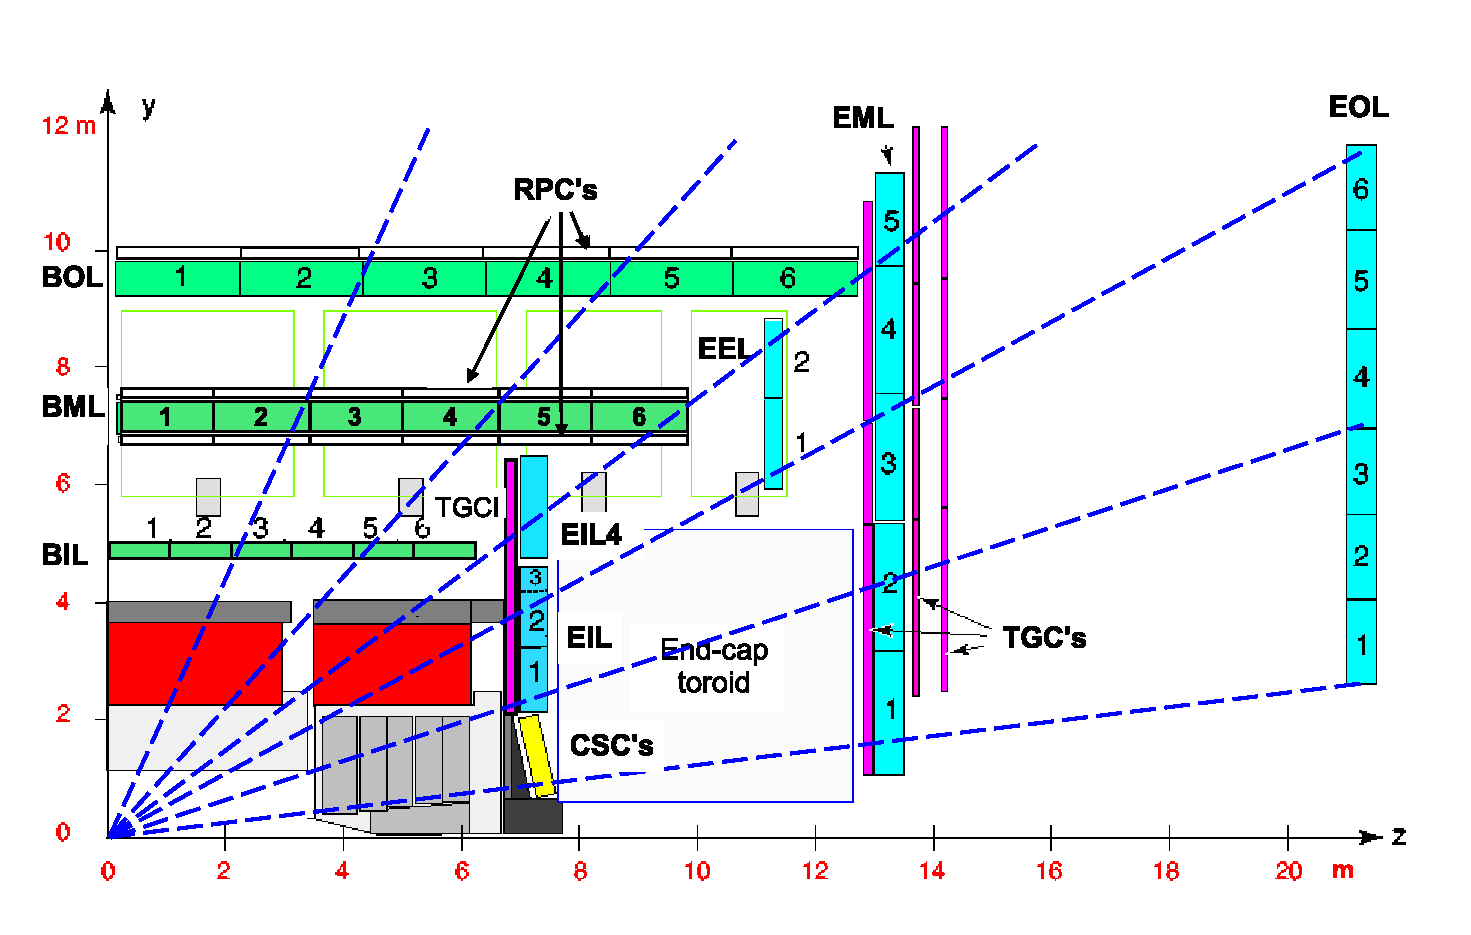
\includegraphics{plots/Chap2/Muon_rz_large_sect_6.eps}
    }
  \end{center}
  \caption[Muon system cross section.]
      {\small Cross-section of the muon system in a plane containing the beam axis (bending plane).  The light green and light blue cells are the MDTs, the yellow cell represets the CSCs, the light purple lines are the TGCs and the labeled black lines are the RPC's.  }
%Infinite-momentum muons would propagate along straight trajectories which are illustrated by the dashed lines and typically traverse three muon stations~\cite{JOIATLAS}.}
  \label{MuonSpectroFig}
\end{figure}

\gls{MDT}'s are used to make the position measurements in the outer two layers of the muon spectrometer over the full eta range ($\mid\eta\mid<$ 2.7), and they are also used in all but the most forward portion of the innermost layer ($\mid\eta\mid<$ 2.0).  
MDTs make use of the trail of ionized particles left behind as a charged particle passes through a gas in a similar way to the TRT (see Sec.~\ref{Sec.ID}), where the gas used here is a 93/7 mixture of Ar/CO$_2$~\cite{JOIATLAS}.  
The most forward region of the inner most layer of the endcaps experiences larger particle rates than is generally considered safe for operating MDTs (greater than 150 Hz/cm$^2$).  
For this reason this region uses \gls{CSC}'s, which have higher time and space resolution as well as lower neutron sensitivity.  
\gls{CSC}'s consist of an array of positively charged anode wires crossed with a series of negatively charged cathode plates all immersed in an active gases medium (80/20 Ar/CO$_2$).  
Charged particles ionize this gas and the electrons/ions are collected on the anodes/cathodes, providing measurements in both directions.  

The MS also contains additional detectors to be used for triggering (see Sec.~\ref{Trig}).  
In the central region ($\mid\eta\mid < 1.05$) three layers of \gls{RPC}'s are used (two sandwiching the central station and a third either on the inside or the outside of the third station.  
\gls{RPC}'s contain no wires and consist of two parallel charged plates surrounding an active gaseous medium (94.7/5/0.3 of C$_2$H$_2$F$_4$/Iso-C$_4$H$_10$/DF$_6$), where charged particles ionize the gas and the electrons are collected on the anode plate.   
The forward region ($1.05<\mid\eta\mid < 1.4$) has additional complications with regards to triggering compared to the central region (larger momentum for the given transverse momentum, inhomogeneities in the magnetic field, higher occupancy), motivating the use of \gls{TGC}'s which are better suited to handle this environment.  
\gls{TGC}'s consist of a number of parallel anode wires between two cathode plates, immersed in an active gas (55/45 CO$_2$n-pentane).  
Three layers of TGC are used in the forward region, organized around the second muon stations (see Fig.~\ref{MuonSpectroFig}).  
\gls{TGC}'s are distinguished from \gls{MPC}'s (not in ATLAS) by having a wire to cathode distance (1.4 mm in this case) smaller than their wire to wire distance (1.8 mm in this case).  

 

\subsection{Triggers}
\label{Trig}
During both 2015 and 2016 the LHC used a beam bunch spacing of 25~ns.  
This resulted in crossing rates of 40~MHz at the centre of the ATLAS detector.  
With each event potentially taking up to 2 MB to store, recording, storing, and analyzing all of these data can be a problem.  
Moreover, the large majority of the collisions are elastic collisions or low $p_{\mathrm T}$ dijet events which are of little interest in this high energy environment.  
The solution to this problem is to only record a certain fraction of the total number of events that have been produced.  
This must be done in a way that maximizes the number of rare events of interest recorded while simultaneously removing as many low interest events as possible.  
The triggering system uses a combination of hardware and software tools to perform this task~\cite{Run2Triggers}.  

The trigger system consists of two parts the first being the \gls{L1} trigger.  
The L1 trigger is hardware based and reduces the number of events to be considered from 40 MHz per second down to 100 kHz.  
It uses a courser object definition than the full event reconstruction.  
Selections can still be made based on energy thresholds for given objects, as well as more topological information like particle isolation requirements or a specified range for the invariant mass of a combination of objects.  

The second stage of the trigger system, which is implemented on a software computer farm, is known as the high-level trigger, or HLT.  
In the HLT some full offline-like unseeded reconstruction algorithms can be run, including topoclustering (see Sec.~\ref{Sec:Topocluster}) and muon reconstruction.  
This is not always the case.  
For example L1 tracking information is used to seed tracks in the HLT to reduce the reconstruction time.  
The HLT is designed to reduce the event rate from the 100 kHz output of the L1 trigger down to 600 Hz, which can be increased to 1-1.5 kHz at peak luminosities.  
Events that pass the HLT criteria are recorded on computer tape for subsequent analysis.   

While these triggers can be very efficient at selecting relatively rare more ``interesting'' events to be recorded for future study, not all event topologies desired by the various physics groups in the ATLAS collaboration are infrequent enough that every instance of that event can be stored.  
In these cases, only a randomly selected, but fixed-fraction, subset of the events is stored for subsequent analysis.  
This is called prescaling.  
The true number of events of these types which have actually occurred can then be determined using the random acceptance rate.  
 
 
 





